
\documentclass[sigchi]{acmart}

\settopmatter{printacmref=false, printccs=true, printfolios=true}
%%
%% \BibTeX command to typeset BibTeX logo in the docs
\AtBeginDocument{%
  \providecommand\BibTeX{{%
    \normalfont B\kern-0.5em{\scshape i\kern-0.25em b}\kern-0.8em\TeX}}}

%% Rights management information.  This information is sent to you
%% when you complete the rights form.  These commands have SAMPLE
%% values in them; it is your responsibility as an author to replace
%% the commands and values with those provided to you when you
%% complete the rights form.
\setcopyright{none}
%\copyrightyear{none}
\acmYear{2021}
\acmDOI{}

%% These commands are for a PROCEEDINGS abstract or paper.
\acmConference[Technical Report]{May}{{\today}}{Cologne, Germany}
\acmBooktitle{}
\acmPrice{}
\acmISBN{}

\usepackage{float}
\usepackage{subfig}
\usepackage[english]{babel}
\begin{document}

\title{The impact of the avatar representation on team trust and effectiveness in a shared virtual environment.}

\author{Hannes Hinrichs}
\email{hhinrich@smail.th-koeln.de}
\affiliation{%
  \institution{TH-Köln}
  \city{Cologne}
  \country{Germany}
}

\begin{abstract}
This paper investigates the impact of the avatar representation on team trust and effectiveness in a shared virtual environment. To answer these questions, a quantitative study was conducted in which different participants in a three-person team performed a collaborative task in a shared virtual environment. The first question here is whether an inverse-kinematic human-like representation or an abstract non-human-like representation is more effective in generating trust in a newly formed virtual team. The second question addresses whether the trust formed by the different representations influences the effectiveness of the virtual team. No significant differences in effectiveness were found between the teams. The results of the study also show that in the threeperson team significantly more trust was built with non humanlike avatars. Furthermore, with non-human-like avatars there was a significant relationship between the cognitive trust formed and teameffectiveness. This means that the simplicity of a non-human-like avatar in a newly formed team in a shared virtual environment can be effective in creating a trusting work atmosphere.
\end{abstract}

\keywords{Virtual-Reality, Trust, Team formation, Virtual Teams, Avatar}

%% A "teaser" image appears between the author and affiliation
%% information and the body of the document, and typically spans the
%% page.
\begin{teaserfigure}
  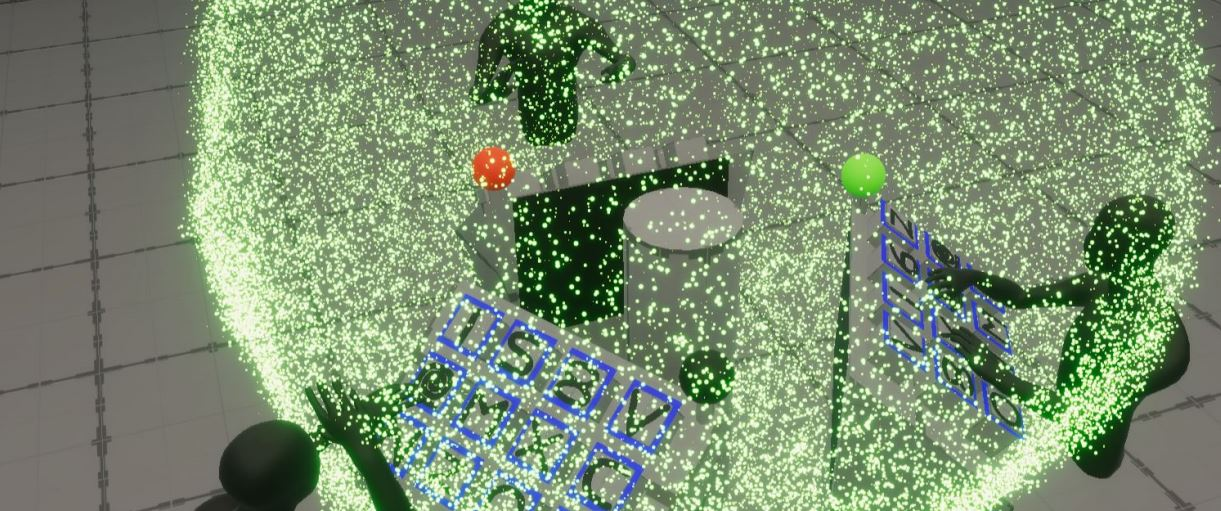
\includegraphics[width=\textwidth]{Abbildungen/RoundSuccsessful2}
  \caption{This figure represents the developed Shared-Virual-Environment with the participants infront of there Podests. A green sphere appears clearly visible when a round is successfully completed.}
  \Description{This figure represents the developed Shared-Virual-Environment. The green sphere appears clearly visible for all participants when a round is successfully completed.}
  \label{fig:teaser}
\end{teaserfigure}

%%
%% This command processes the author and affiliation and title
%% information and builds the first part of the formatted document.
\maketitle

\section{INTRODUCTION}
With advancing technological development, digital communication is becoming more and more central. Companies around the world have long relied on overcoming spatial and temporal boundaries.
New generations of social networking systems are being created on the premise of improving communication to remote individuals.
Einsatzfelder sind beispielsweise die Mobil- und Internettelefonie, die FOIP/VOIP- Telefonkonferenzen oder die sozialen virtuellen 3D- Umgebungen.
All these technologies share the goal of enhancing social presence, allowing users to gain some degree of insight and the cognitive and affective states of the interaction partner \citep[S. 407–447]{biocca2001plugging}.
Employees in an organization are very often not in the same place, yet many companies still want their teams to be effective \citep[S. 791-792]{jarvenpaa1999communication}. \textit{Virtual teams} can provide a remedy here. 
Before the Corona pandemic, in Q2 2020, 4\% of all employees in Germany worked from home. This share has risen to 24\% over the course of the year - as of 01.01.2021 - and theoretically 80\% of employees could work from home. \citep{statistaCorona2020}. As a result of this development, companies have inevitably had to look at how virtual teams work.
When a virtual team meets in a virtual reality environment, avatars can be used to represent the individual. These are used to interact and communicate with other participants in the shared virtual environment.
\textit{Virtual teams} are often short-lived, which creates a deficit in the trust formed with team members.
Working in a geographically separated team that does not trust each other or does not work together properly inhibits its performance. \citep[S. 98-107]{huang1998supporting} \citep[S. 399-417]{turoff1993distributed}. This paper aims to better understand the construct of trust in the virtual world and how to deal with it in order to work more effectively in a virtual team.
The goal of the study was to find out which type of representation builds more trust in a virtual team. The focus was on the two avatar conditions "human-like" and "non-human-like" in order to analyze whether there is a correlation between the "cognitive trust" formed in the team and the "team effectiveness" under different avatar representation types during collaboration.
In addition, the focus is on the general propensity to trust of individual trial participants to investigate whether the \textit{general propensity to trust} has an influence on the \textit{team effectiveness} and the \textit{cognitive trust} with respect to the different avatar representations. For this purpose, a three-person team, whose members did not know each other, competed in a collaborative task in a shared virtual environment.

\section{RELEATED WORK}
This section provides an overview of the topic of trust and teams.
\subsection{TRUST}
The most widely used definition of trust comes from Meyer et al. \citep[S. 712]{mayer1995integrative}. They define trust as:
\begin{quote} \grqq{}is the willingness of a party to be vulnerable to the actions of another party based on the expectation that the other will perform a particular action important to the trustor, irrespective of the ability to monitor or control that other party.\grqq{} \end{quote}

Trust is not considered static and one-sided. A person can not only \textit{trust} or \textit{not trust}.. Trust is a dynamic construct that changes over time. It can be divided into a formation, stabilization and decreasing phase \citep[S. 396]{rousseau1998not}.

During the early phase of trust building, it is decided whether a relationship will be maintained or not. Subconsciously, a feeling of confidence and security or a feeling of tension, doubt and skepticism towards the interaction partner is formed.
It does not matter whether the decision is made to trust someone or not. The strength of the positive or negative subconscious sense of trust influences the effectiveness of collaboration. Trust can make it easy or difficult to work with another person and to achieve goals in a group or team \citep[S. 405-406]{bigley1998straining}.

The initial phase of trust formation affects the \textit{cognitive} Trust, which has a strong influence on the developing trust model about a person.
Opinions and assumptions formed early on thus strongly shape future opinions about the trustee \citep[pp. 461-462]{baldwin1992relational}.

Many psychologists studying trust now assume that \textit{interpersonal} trust consists of a two-dimensional construct \citep{johnson2005cognitive}; \citep{cook1980new}. Thus, Mooradian et al. consider that trust is viewed as a \textit{trait} or as a \textit{state} \citep[pp. 524-525]{mooradian2006trusts}.

\subsubsection{TRUST AS A TRAIT }
Trust as a trait reflects a person's attitude toward trust. This attitude toward trust is long-lasting and is not quickly built up or broken down. Es ist das Grundlevel an Vertrauen, das eine Person in eine neue zwischenmenschliche Beziehung mitbringt \citep[S. 11]{couch1996assessment}. 

\textit{General trust} implies that most persons can be trusted, or that in the case of general distrust, persons cannot be trusted \citep[p. 409]{stolle2002trusting}.

The \textit{general trust} is not situation-dependent, but represents a longer-term constant based on the basic trust of a person. In this context, it is composed of the individual characteristic of an individual person's propensity to trust as well as the basic mood toward people in general \citep[p. 11]{couch1996assessment}.

\subsubsection{TRUST AS A STATE}
If \textit{trust as a state} is considered, this trust may change over time \citep[p. 712]{mayer1995integrative}.

According to the study by Lewis et al. \citep[pp. 970-971]{lewis1985trust}, trust is based on
\begin{quote} \grqq{}a cognitive process which discriminates among persons and institutions that are trustworthy, distrusted, and unknown. In this sense, we cognitively choose whom we will trust in which respects and under which circumstances, and we base the choice on what we take to be "good reasons", constituting evidence of trustworthiness.\grqq{} \citep[S. 970]{lewis1985trust}.\end{quote}

\textit{Cognitive Trust} is based on a logic we define rather than an emotional component. It can be established in the short term and is easily vulnerable to external influences \citep[p. 970]{lewis1985trust}. 

Thus, individual \textit{cognitive trust} is based on \textit{conviction in the abilities or reliability of another} \citep[S. 30]{mcallister1995affect}.

\subsection{VIRTUAL TEAMS}
A Team is defined as \begin{quote}\grqq{}a small number of people with complementary skills who are equally committed to a common purpose, goals, and working approach\grqq{} \citep[S. 2]{zenun2007effects}. \end{quote}

\textit{Virtual teams} share many characteristics of traditional \textit{teams}, but have a virtual component \citep[S. 270]{schweitzer2010conceptualizing}.
According to Schweitzer et al, \textit{virtual team} have come into being due to communication technology and work spatially separated, across borders, and asynchronously \citep[p. 270]{schweitzer2010conceptualizing}.

The challenge of a \textit{virtual team} arises from the different cultures, distances and time zones of the team members. If a \textit{virtual team} trusts each other, the disadvantage of different cultures, distances and time zones can become an advantage. Cultural diversity is promoted and new patterns of behavior are acquired, fostering new, creative ways of working. Through these factors it is possible to work and think more innovatively \citep{dyer1995team} \citep[S. 405-416]{milliken1996searching}.

Virtuality is viewed as a continuum where each team has some degree of virtuality. This continuum ranges from face-to-face to complete communication only via communication technology \citep{martins2004virtual} (see \textit{Figure \ref{virtualTeamsVirtuality}}).

\begin{figure}[h]
  \centering
 	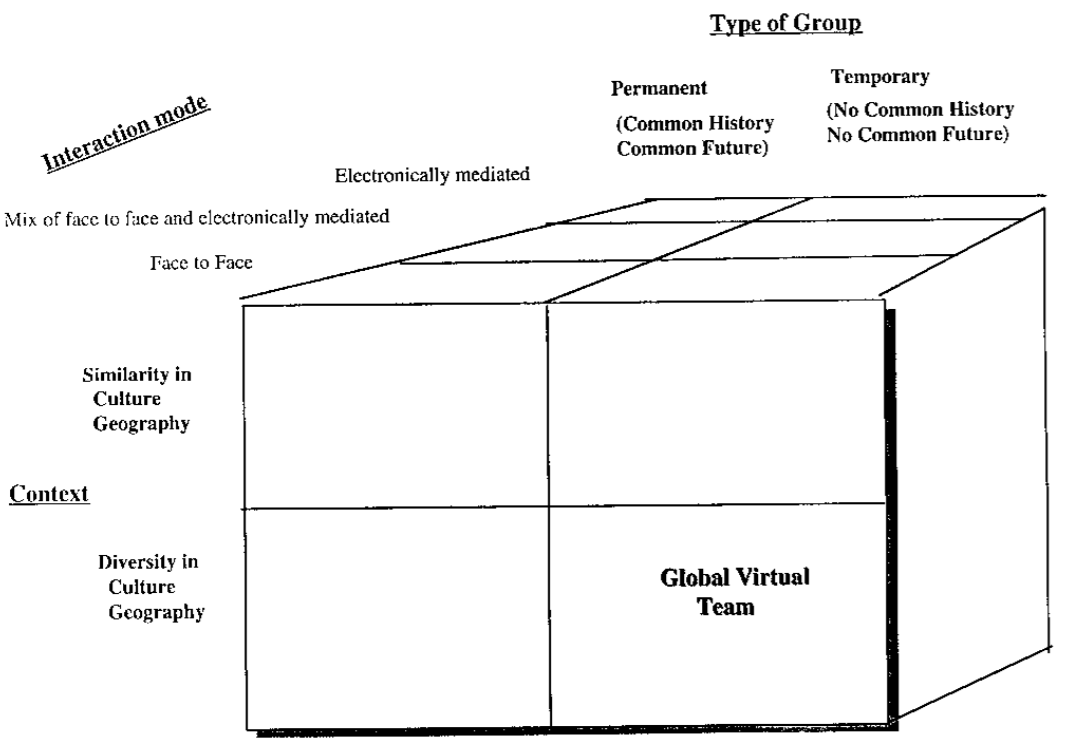
\includegraphics[width=\linewidth]{Abbildungen/GlobalVirtualTeam.PNG}	
			\caption[Virtuality of a virtual team]{Degree of virtuality that a team must reach to be considered a \textit{virtual team} \citep{jarvenpaa1999communication}.}
			\label{virtualTeamsVirtuality}
\end{figure}

Members of a \textit{virtual team} have fewer opportunities to see each other, interact or resolve conflicts, unlike traditionally formed teams. Respect and trust are the basic building blocks of a \textit{virtual team}. The effectiveness of a team is a direct consequence of this \citep[p. 378]{ren2007applying}.

\paragraph{VIRTUAL TEAMS AND TEAMEFFECTIVENESS}

Schweitzer et al. \citep{schweitzer2010conceptualizing} assumes that traditionally formed teams are more effective than \textit{virtual teams} and that \textit{team effectiveness} decreases the higher the degree of virtuality (see \textit{fig \ref{virtualTeamsVirtuality}}).
This opinion is also shared by Becker et al. According to them, the exchange of information content and the building of trust suffers due to increasing virtuality and the same effectiveness as in a face-to-face team cannot be achieved \citep{becker2002fuhrung}.

Previous studies have found positive correlations \citep{davis2000trusted}, no correlations \citep{hertel2004managing}, and negative correlations \citep{dirks1999effects} between trust and \textit{team effectiveness} in \textit{virtual teams}.

Despite the contradictory results of studies, the general opinion is that trust has a positive influence on \textit{team effectiveness} \citep{en2016trust}. 
Trust in one's team helps to block out one's own uncertainties in order to work more safely and effectively \citep{de2010does}. Furthermore, existing trust in one's team creates a greater interest in the team members, which unlocks synergy effects and enables more direct and effective interaction \citep{dirks1999effects}. 

\subsection{AVATARS AND TRUST}
George et al. \citep{george2018trusting} analyzed in their research whether more trust can be established with human-like or robotic avatars in a shared virtual environment. They found no significant difference in trustworthiness. However, a greater sense of commonality was found when interacting with a human-like avatar.

Riedl et al. \citep{riedl2014trusting} conducted a study on trust building among humans compared to avatars with human-like faces. They found that people find it easier to trust a real person than an avatar with a human-like face. According to them, trust is built between humans at the same rate as between humans and avatars.
This assumption was also confirmed by Bente et al. \citep[S. 54-59]{bente2004social}. They found that in a \textit{shared-virtual-environment} less \textit{cognitive trust} is built up towards avatars than in face-to-face, telephone and chat communications.

\section{METHOD}

A \textit{A/B testing} in combination with an inductive quantitative research design was chosen.
Group A was assigned the condition humanlike, while group B was assigned the condition non-humanlike (\textit{Figure \ref{Avatars}}). Participants were randomly assigned to groups and conditions. 

The analyses in this study were conducted at different levels.
Since participants work as a team and different teams have different conditions, some correlations are conducted at \textit{condition level} and some are conducted at \textit{team level}.

The \textit{individual level} is about an individual person, while the \textit{condition level} distinguishes between the conditions \textit{humanlike} and \textit{non-humanlike}.

The condition level can be divided into teams of 3 persons each. This division is called \textit{TeamLevel} and makes it possible to make assumptions about the team. 
The \textit{Figure \ref{DifferentLevels}} shows the hierarchy of the different levels.

\begin{figure}[h]
  \centering
 		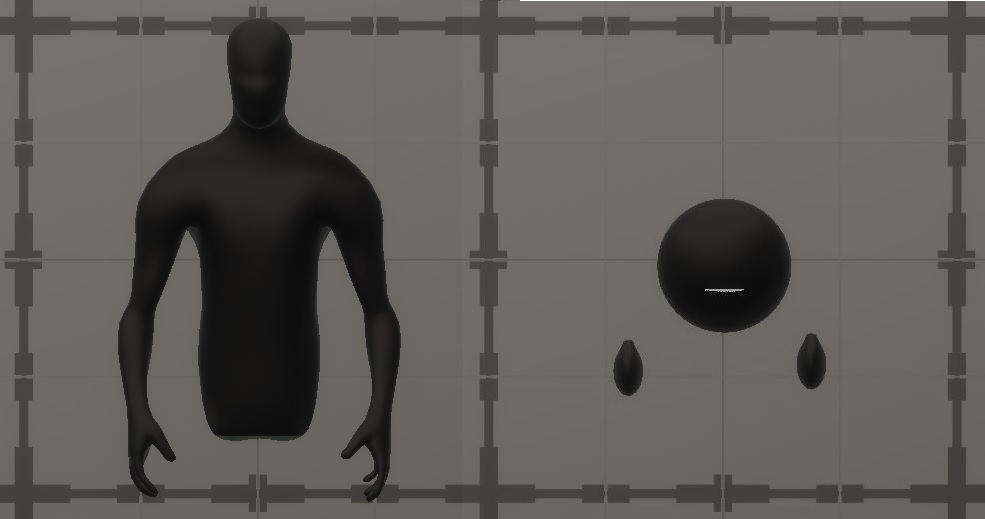
\includegraphics[width=0.60\linewidth]{Abbildungen/Avatars.JPG}
			\caption[The avatars]{This figure shows the avatars used during the experiment. Left: \textit{humanlike} avatar and right: \textit{non-humanlike} avatar.}
			\label{Avatars}
\end{figure}	

\begin{figure}[h]
  \centering
 		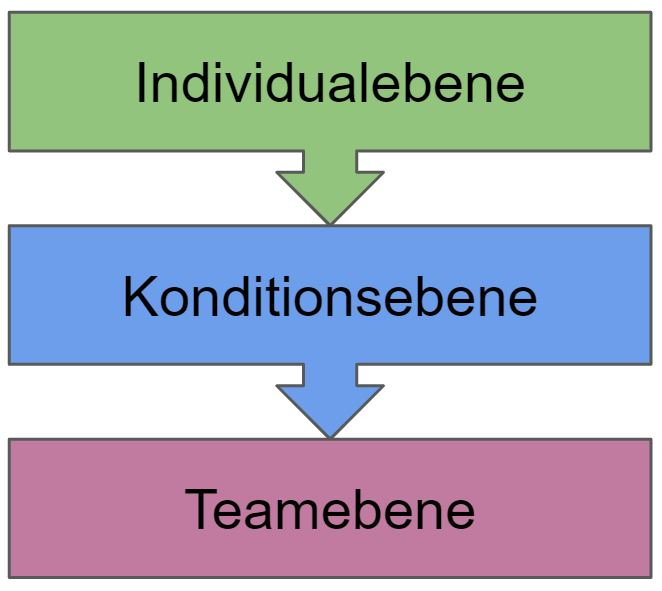
\includegraphics[width=0.40\linewidth]{Abbildungen/DifferentLevels.JPG}	
			\caption[The hierarchy levels]{The hierarchy of individual-level, condition-level and team-level.}
			\label{DifferentLevels}
\end{figure}	
	
Using a self-constructed theory-based framework (see \textit{Figure \ref{Trial Hypotheses}}), the following hypotheses were formulated :

\textbf{H1}: The mean values of the obtained \textit{cognitive confidence scores} differ significantly from each other between the \textit{humanlike} and \textit{non-humanlike} conditions.

\textbf{H2}: The higher the achieved \textit{general trust score} of a person, the higher the achieved \textit{cognitive trust score} of a person.

\textbf{H3}: The correlation between the \textit{cognitive trust score of teams} and the \textit{team effectiveness} with the condition \textit{humanlike} is stronger than that of teams with the condition \textit{non-humanlike}.

\textbf{H4}: The mean values of \textit{team effectiveness} differ significantly from each other between the \textit{humanlike} and \textit{non-humanlike} conditions.

\textbf{H5}: The correlation between the \textit{general trust score of a team} and the \textit{team effectiveness} with the condition \textit{humanlike} is stronger than that of teams with the condition \textit{non-humanlike}.

\begin{figure}[H]
		\begin{footnotesize}
			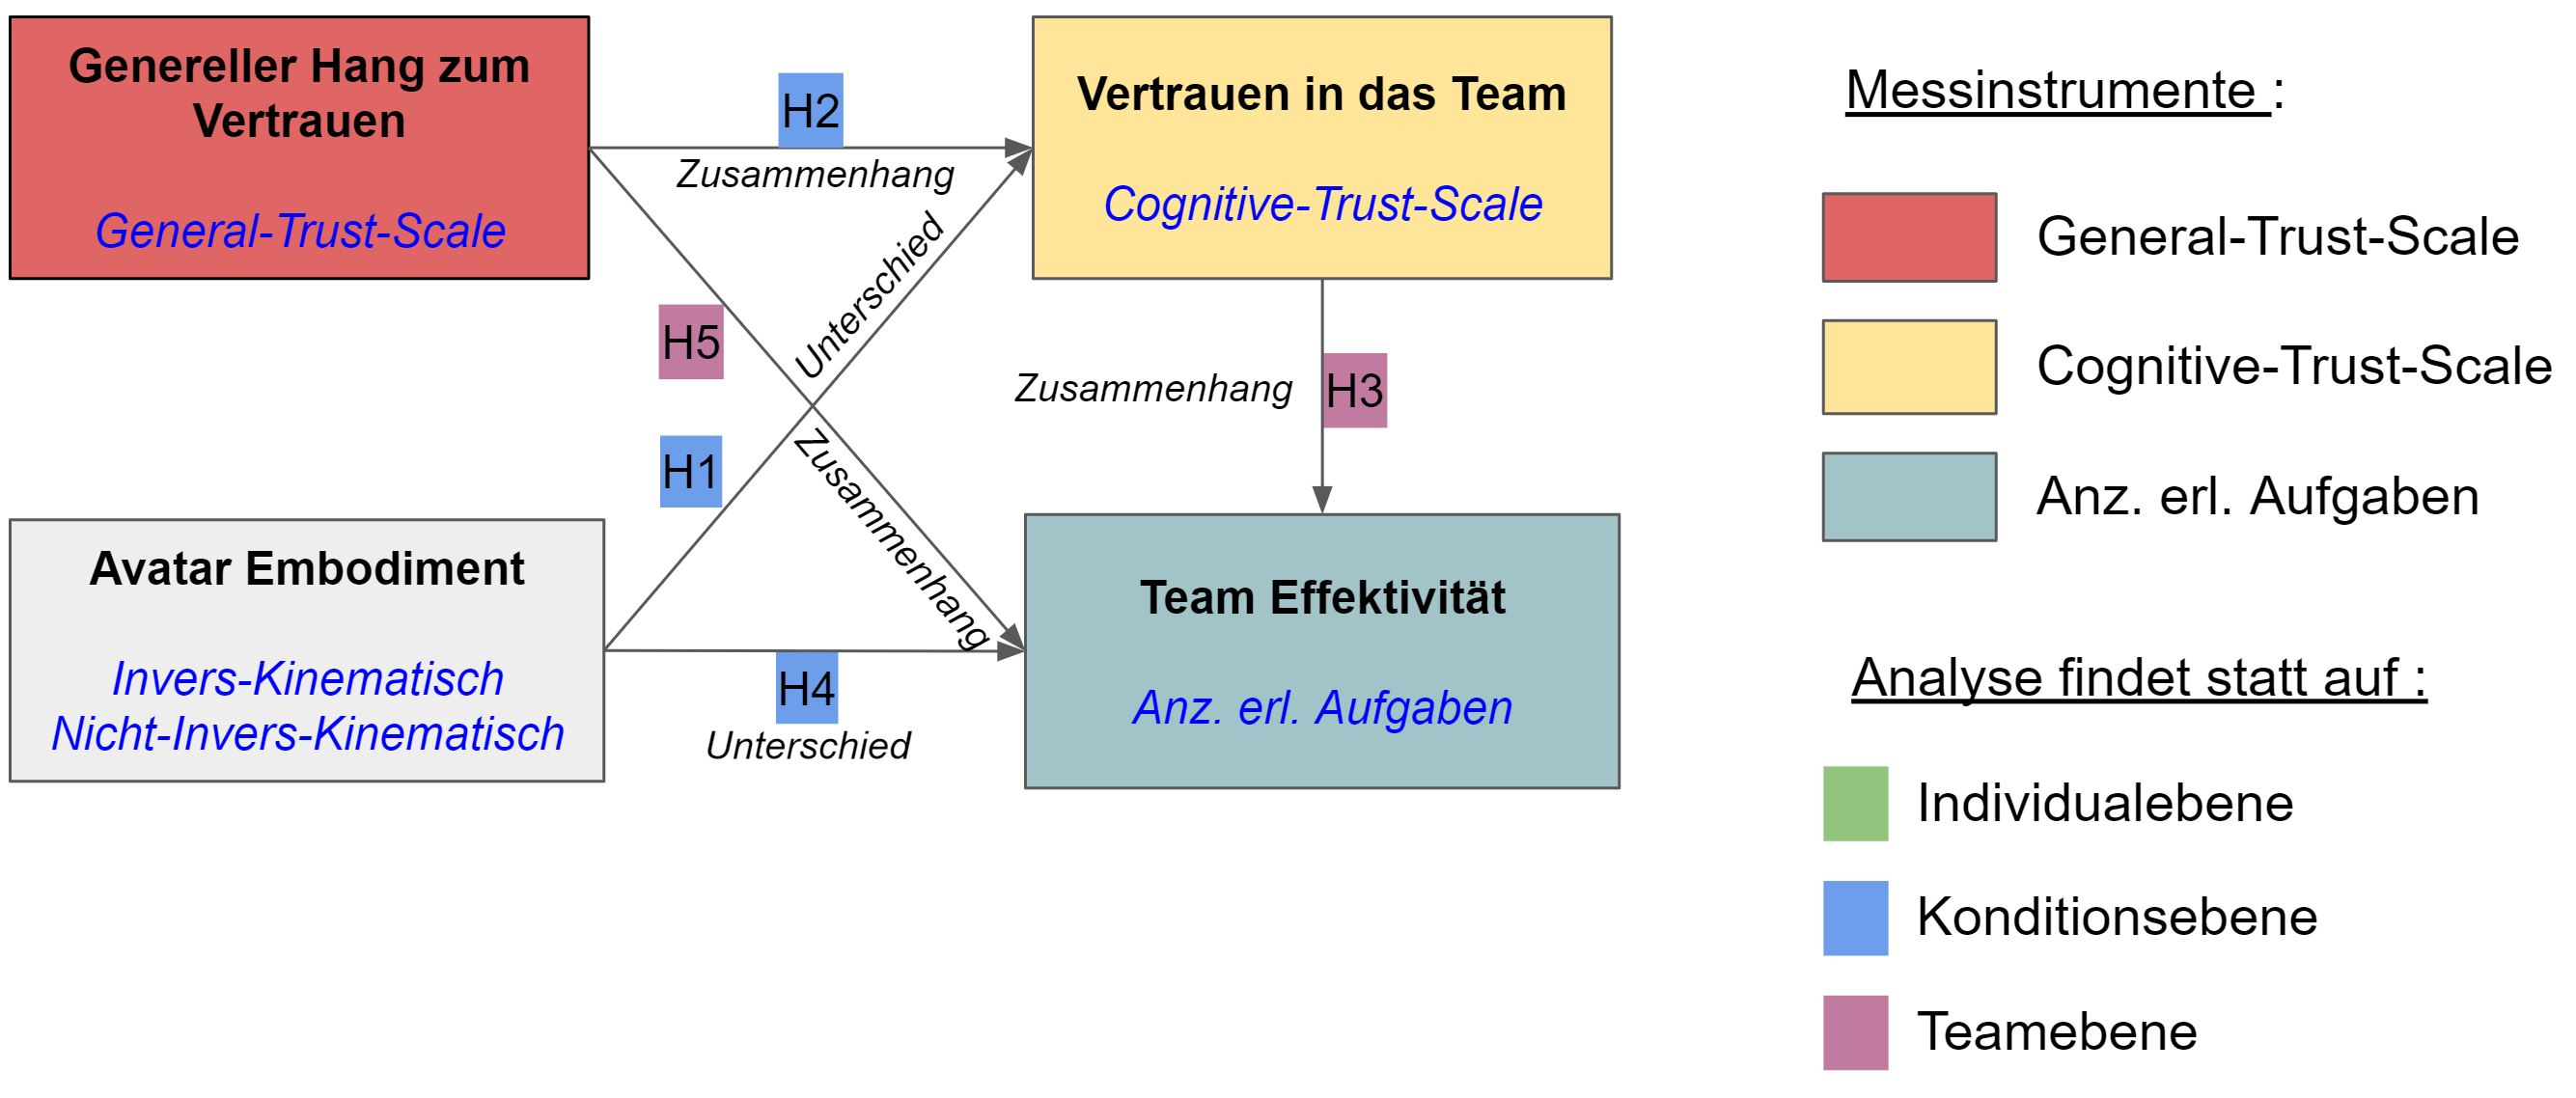
\includegraphics[width=\linewidth]{Abbildungen/Versuchshypothesen_02.JPG}		
			\caption[The self-constructed framework of experimental hypotheses]{This framework illustrates the interrelationships of the posed hypotheses.}
			\label{Versuchshypothesen}
		\end{footnotesize}
	\end{figure}	

General trust in this study refers to the extent to which participants tend to give others the benefit of the doubt. \citep[S. 30]{mcallister1995affect}.
\textit{Cognitive trust} refers to \textit{conviction} in the abilities or in the reliability of another \citep[S. 30]{mcallister1995affect}.
The \textit{team effectiveness} is measured by the number of rounds completed by the team during the experiment.

%\subsection{MEASURING METHODS}
\begin{table*}
  \caption{MEASURING METHODS}
  \label{tab:commands}
  \begin{tabular}{llcr}
    \toprule
    Scale & What was measured? & $\alpha$ & Likert-Points \\
    \midrule
    \texttt{General-Trust-Scale \citep{couch1996assessment}} & Propensity to trust of the individual participants & ,91 & 1-7 \\
    
    \texttt{Cognitive-Trust-Scale \citep[S. 37]{mcallister1995affect}} &Built up \textit{cognitive trust} during the experiment & ,91 & 1-5\\
    
     \texttt{\textit{Quality of team communication} \citep[S. 1049]{gonzalez2014climate}} & Perceived quality of team communication & ,76 & 1-5 \\
     
      \texttt{\textit{Perceived team effectiveness}\citep[S. 469]{gibson2003team}} & Extent of the perceived team effectiveness & ,62-,88 & 1-7\\
          
       \texttt{NASA-TLX\citep{NASATLX}} & Task load during the experiment & ,84 &1-21  \\
       
       \texttt{IPQ \citep{IPQ}} & The sense of presence & ,85 & 1-7 \\
       
        \texttt{\textit{Co-Präsenz} \citep[S. 487]{nowak2003effect}} &  Co-, Social-, Telepresence & ,78-,90 & 1-7; 1-10 \\
    \bottomrule
  \end{tabular}
\end{table*}

\subsection{PARTICIPANTS}

The participants were acquired in two ways. On the one hand, people in the circle of acquaintances were approached, who would be provided with the necessary hardware. Secondly, participants were sought in various forums (e.g. VRForum.de, Computerbase.de, Hardwareluxx.de, etc.). Furthermore, participants were acquired with the help of various social networks related to VR as well as random WhatsApp chat groups with 50 or more members.

To participate in the experiment, participants needed a fully functioning SteamVR, Windows Mixed Reality, or Oculus Rift/Rift-S head-mounted display with compatible controllers, as well as a powerful VR-enabled PC. The experimenter used a PC without a head-mounted display to control and manage the experiment from outside.

\subsection{PROCEDURE AND IMPLEMENTATION}
To conduct the experiment, a shared virtual environment was developed in which three team members could see each other as avatars and interact with each other. The shared virtual environment has been developed with Unity 2019.4.3f1 and the HD render pipeline. To ensure real-time communication between clients, the multiplayer framework \textit{Normcore v2.0}\footnote{www.Normcore.io} was used.

Three people were placed in each time slot to form a team. The participants were \textit{not} introduced face-to-face and saw themselves only as a representation of an avatar.
The test lasted 35 minutes and was divided into
		\begin{itemize}
			\item 5 minutes pre-questionnaire,
			\item 5 minutes video explanation,
			\item 10 minutes experiment,
			\item 15 minutes post-questionnaire.
		\end{itemize}
The pre-questionnaire was used to collect general demographic data from the participants. The explanatory video showed all the relevant mechanics of the experiment. Furthermore, the video explanation ensured that all participating individuals had the same level of information about how the experiment was conducted. During the experimental session, participants had 10 minutes to complete as many rounds as possible as a team. Over the subsequent post-questionnaire, all relevant questionnaires were processed for statistical analysis of the experimental hypothesis. The maximum test duration after starting the experiment was 600 seconds and a maximum of 15 rounds could be completed. The rounds became incrementally more difficult every third round as one symbol was added to the pool of symbols to be guessed.
\textit{Figure \ref{RoundDifficulty}} shows the increasing round difficulty used to measure \textit{team effectiveness} in this experiment.

\begin{figure}[H]
		\begin{footnotesize}
		\centering
			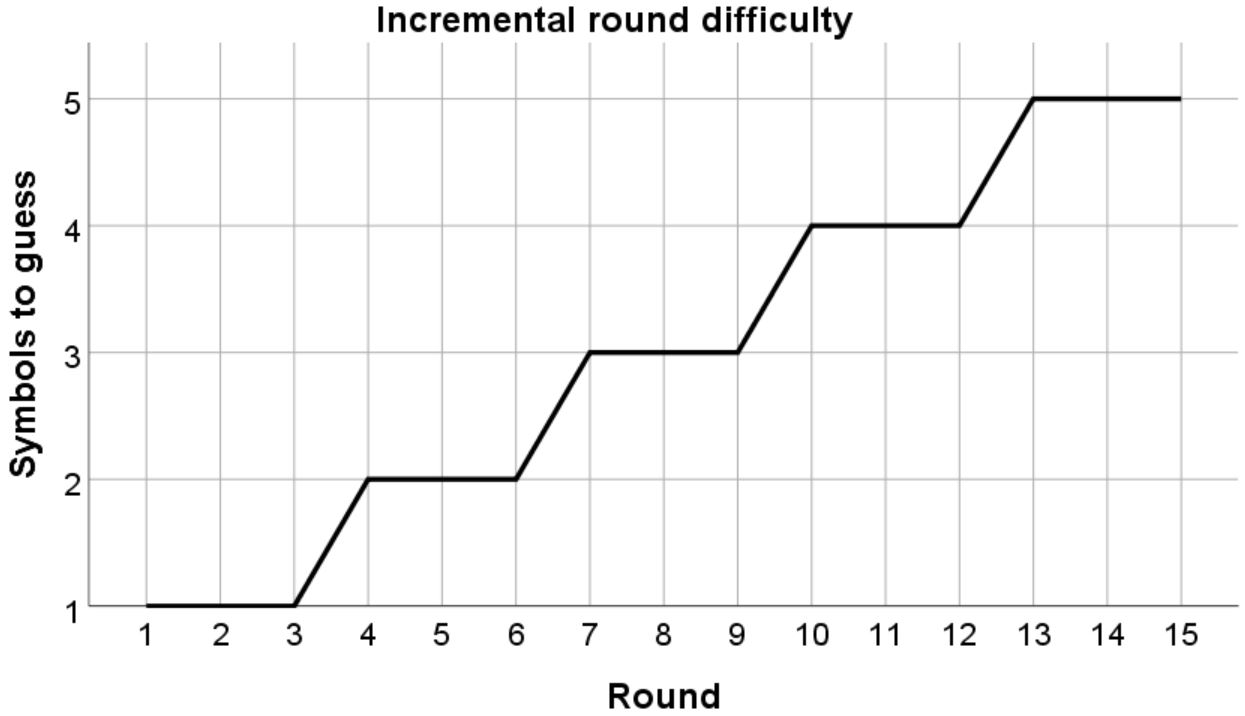
\includegraphics[width=0.9\linewidth]{Abbildungen/RoundDifficulty.JPG}	
			\caption[The difficulty of the rounds]{The increasing difficulty of the symbols to be guessed in the rounds. In rounds 1-3 one symbol had to be guessed, in rounds 3-6 two symbols and so on.}
			\label{RoundDifficulty}
		\end{footnotesize}
	\end{figure}

\subsection{DETAILED TEST EXECUTION}
At the beginning of each new round, players were assigned the color black, green or red.
The player marked black has the task of explaining to his teammates the symbols that are color-coded for him. The other team members had the task to identify the symbols shown by the black player by gesticulation and to log them on their podium. The goal was to correctly identify as many symbols as possible, thereby advancing to higher rounds together.

The symbols on the podium of the player marked in black were color-coded either green, red or green-red. The podiums of the other players also had symbols on them, but these were arranged randomly and had no color markings. The player marked in black now tried to explain the symbols marked in the respective player color in front of him to the other players marked with red and green. If the player just addressed by the black player believed to have recognized a symbol, he logged the symbol by pressing down the matching button on his podium. 

If all the marked symbols were successfully identified and logged in, a bright green ball appeared, indicating the end of a round.
In the next round, another player was clearly marked with black, red or green.
\textit{Figure \ref{AvatareImEinsatz}} shows both avatar conditions \textit{humanlike} (a) and \textit{non-humanlike} (b) during the experimental procedure.
	
\begin{figure}[H]
  \centering
  \subfloat[][]{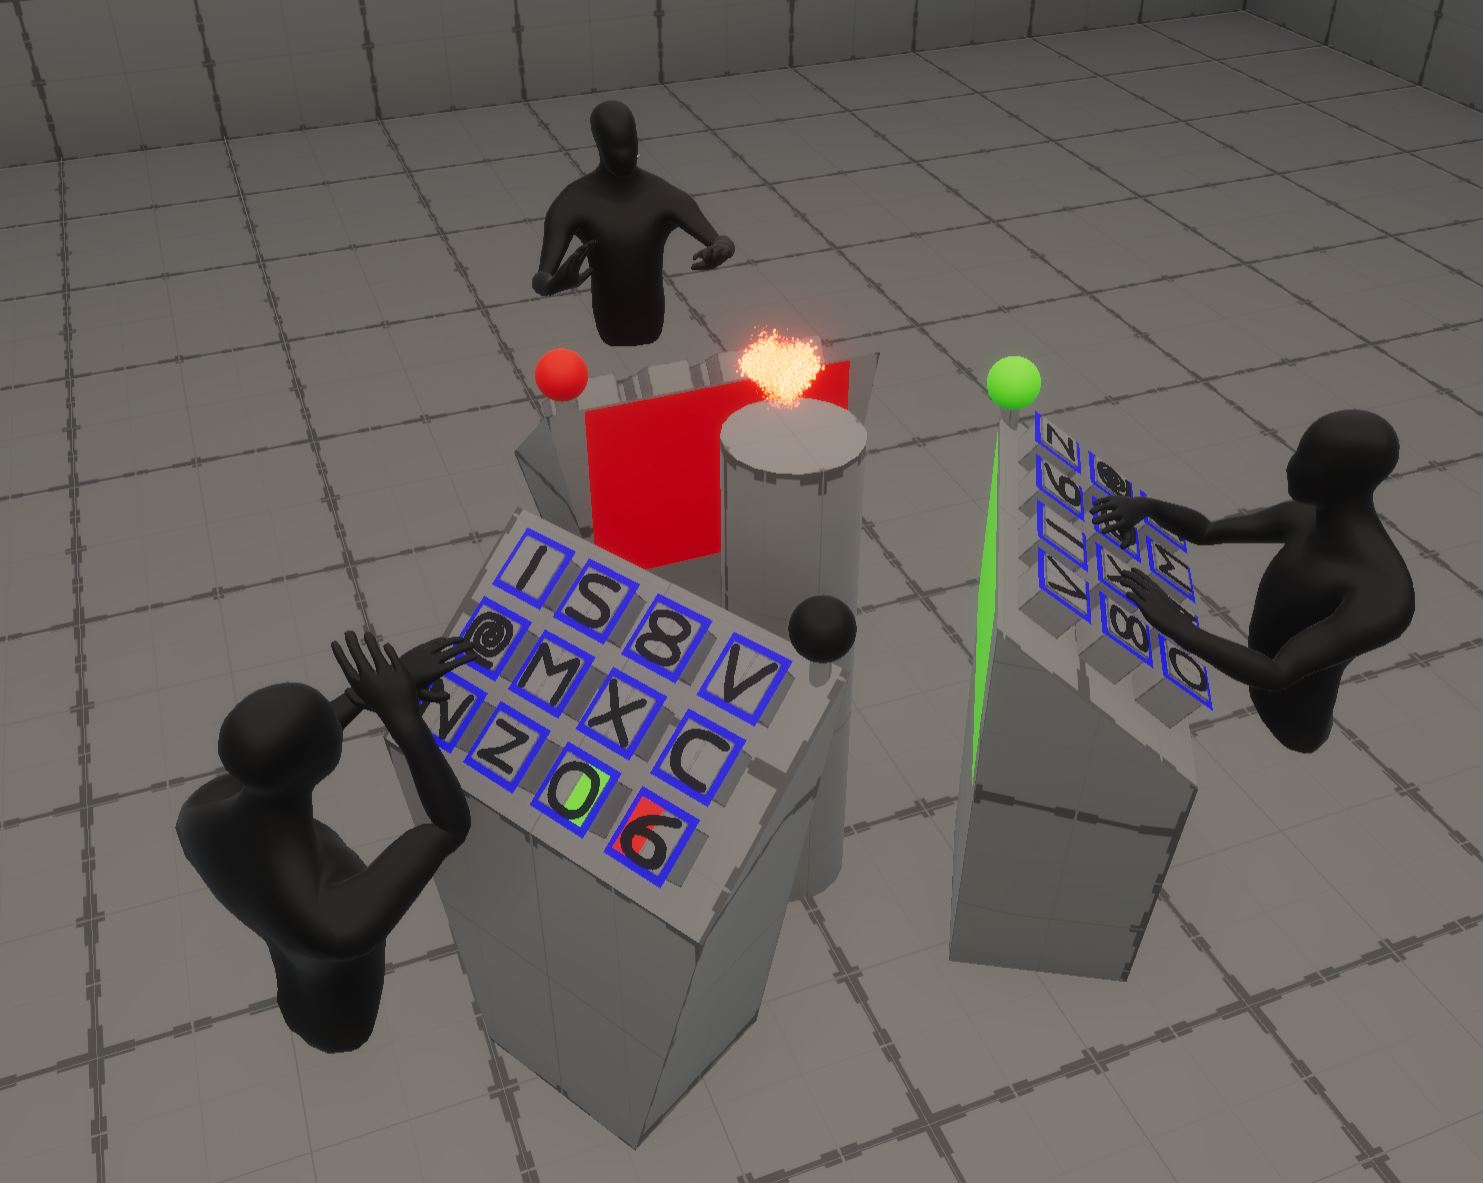
\includegraphics[width=0.41\linewidth]{Abbildungen/Podeste_IK_Avatars.jpg}}
  \qquad
  \subfloat[][]{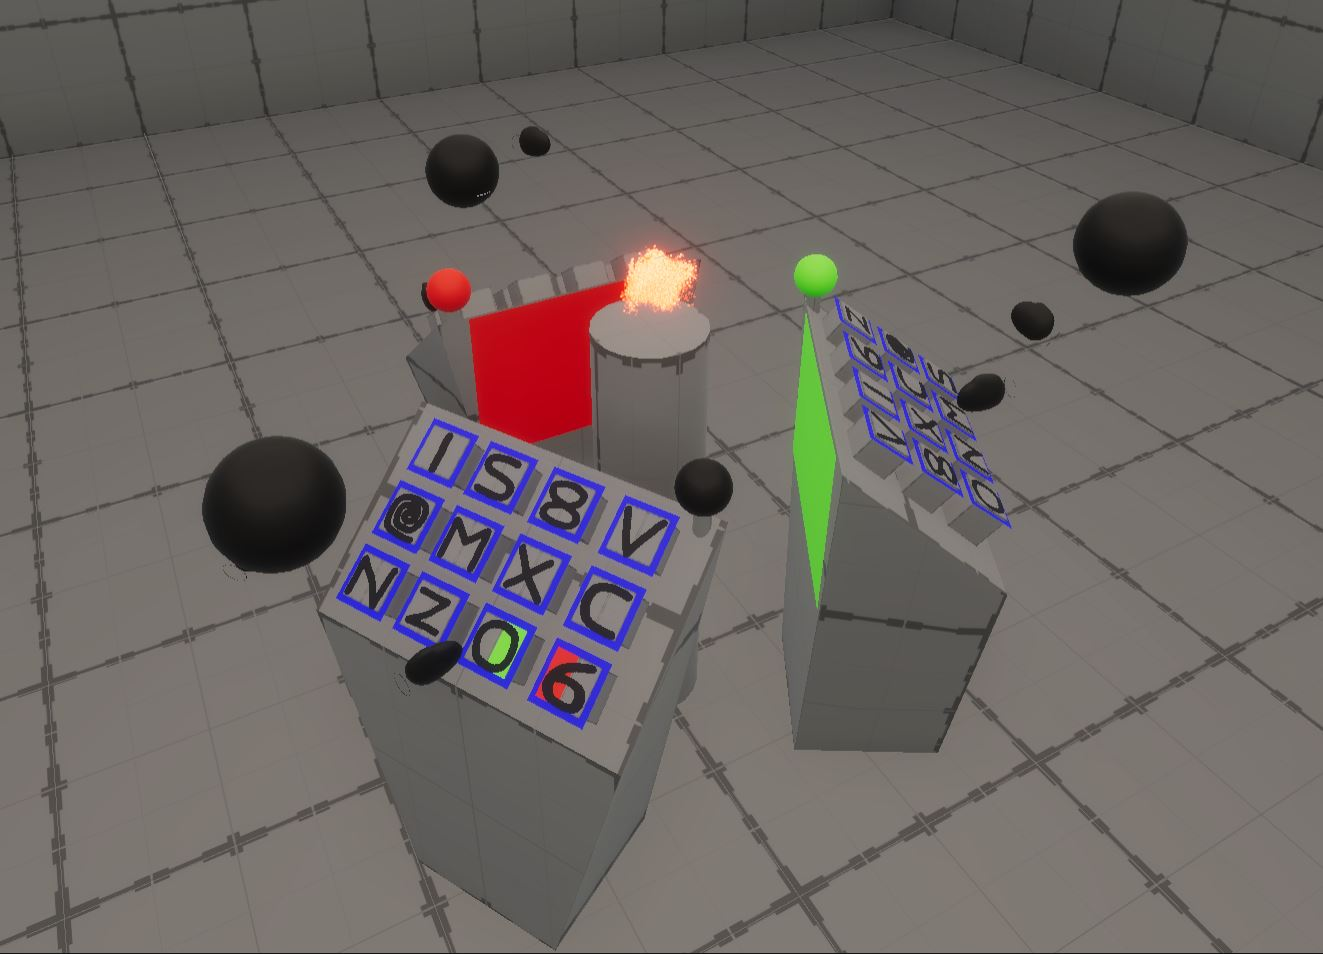
\includegraphics[width=0.45\linewidth]{Abbildungen/Podeste_Non_IK_Avatars.jpg}}
  \caption[The avatars in the experimental environment]{Avatar conditions \textit{humanlike} (a) and \textit{non-humanlike} (b) during the execution of the experiment.}
  \label{AvatareImEinsatz}
\end{figure}

\section{RESULTS}
A total of 30 people participated in the study, making a total of ten teams. Nineteen (63.3\%) individuals were male and 11 (36.7\%) were female. On average, participants were 30 years old $(\bar{x} = 30.13)$, with the 2nd quartile being $28$ years old.

Before the results were analyzed, a Shapiro-Wilk significance test was performed to check for normality.
\subsection{HYPOTHESIS}
%H1
Based on the statistical analysis of hypothesis 1, it can be concluded that different avatar conditions have a \textit{significant} influence on the formed \textit{cognitive trust} (Mann-Whitney-U: $U = 64.000; Z = -2.029; p =.042 < \alpha =.05; r =-.370$). Thereby, participants with the condition \textit{non-humanlike} $(\bar{x} = 4.622)$ formed more \textit{cognitive trust} than participants with the condition \textit{humanlike} $(\bar{x} = 4.188)$. 

%H2
Through the analysis of hypothesis 2, \textit{no evidence} could be found that there is a \textit{significant} correlation between \textit{general trust} and \textit{cognitive trust}. 

%H3
Contrary to the assumption of hypothesis 3, a \textit{significant} relationship was found between the formed \textit{cognitive trust in the team} and the \textit{team effectiveness} with the condition \textit{non-humanlike} (Spearman-Rho: $r =.975$; $p =.005 < \alpha = .05$). This correlation differs according to Fisher Z-score for independent samples ($Z=-1.977$), \textit{significant} ($p =.024 < \alpha = .05$) from that correlation of the condition \textit{humanlike}.
 
%H4
During the analysis of hypothesis 4, it was found that \textit{team effectiveness} \textit{not significant} differs from each other due to different avatar conditions (Mann-Whitney U: $U = 103.500; Z = -.377; p =.706 > \alpha = .05; r = -.060$). An average team effectiveness of $\bar(x) = 9$ was found for both avatar conditions.

%H5
Based on the analysis of hypothesis 5, there is \textit{no evidence} that there is a \textit{significant} correlation between a person's \textit{propensity to trust} and \textit{team effectiveness} in a \textit{virtual team}.

\subsection{SUBJECTIVE DATA}
During the analysis of the subjective data at the condition level, a \textit{significant} difference of the mean values of team communication (Mann-Whitney-U : $U = 63.500; Z = -2.062; p =.039 < \alpha = .05$) was found. The mean value of the \textit{team communication} of the condition \textit{humanlike} is $\bar{x} = 4.013$, while the mean value of the team communication of the condition \textit{non-humanlike} is $\bar{x} = 4.48$. For both conditions, the tendency of high team communication is evident ($\bar{x} = 4.013$; $\bar{x} = 4.48$ $ > \bar{x} = 3$).

Furthermore, at the condition level of \textit{non-humanlike}, there is a \textit{significant} positive correlation between \textit{cognitive trust} and \textit{perceived team effectiveness} (Spearman-Rho: $r =.869; p =.000 < \alpha = .05$) and \textit{team communication}.

Also, a \textit{significant} positive correlation of the condition \textit{non-humanlike} at the condition level between \textit{cognitive trust} and \textit{team communication} was found (Spearman-Rho: $r =.676; p =.006 < \alpha = .05$).

Moreover, it can be noted that an increased sense of presence (presence ($\bar{x} = 4.446 > 3.5$), telepresence ($\bar{x} = 4.446 > 3.5$) , self-perceived co-presence ($\bar{x} = 3, 827 > 3.5$), perceived co-presence of the other ($\bar{x} = 3.877 > 3.5$), and social presence ($\bar{x} = 6.409 > 5$)) was formed at the condition level during the experimental. Overall the perceived stresslevel was below the average ($\bar{x} = 7 < 11$) and perceived team effectiveness was above average ($\bar{x} = 4.886 > 13.5$).

\section{DISCUSSION}
In this chapter, the results of the study are discussed and limitations are pointed out.

\subsection{BUILDING TRUST THROUGH DIFFERENT AVATAR CONDITIONS}
The results of hypothesis 1 contradict the study by Bente et al. \cite{bente2004social} which suggested that there is a greater increase of \textit{cognitive trust with the condition} \textit{humanlike} than with the condition \textit{non-humanlike}. It is just the opposite according to the statistical analysis, because the participants with the condition \textit{non-humanlike} achieve on average a significantly higher \textit{cognitive trust} score.
One reason for this result could be that the \textit{humanlike} avatar used was affected by the \textit{uncanny valley effect} \footnote{The Uncanny Valley Effect describes the feeling of uneasiness above a certain level of reality \citep[pp. 352-353]{guest2011uncanny}.}.
Furthermore, the inverse kinematics used in this experiment could have been perceived as strange. Misinterpreted gesticulation may also have led to a lower level of trust in the respective counterpart.

\subsection{BUILDING TRUST THROUGH GENERAL TRUST}
The fact that there is no significant correlation between \textit{cognitive trust} and \textit{general trust} in different avatar conditions (hypothesis 2) can also be seen as an advantage.
Thus, it can be surmised that during short-term collaboration in a shared-virtual environment, it is not relevant how high or low a person's \textit{propensity to trust} is. 
Since only the different avatar conditions have a significant impact on the formation of cognitive trust, it can be assumed that \textit{general trust} does not play a major role during a get-to-know phase of a virtual team and can be considered in isolation.

\subsection{TRUST IN THE TEAM AND TEAM EFFECTIVENESS}
Since hypothesis 4 cannot be accepted, but a significant correlation with the condition \textit{non-humanlike} was found in the analysis of hypothesis 3, it must be suspected that the results of hypothesis 3 and hypothesis 4 are either random in nature or the measurement of team effectiveness needs to be improved.
The small sample size of the study could also be a reason why the results of hypothesis 3 and hypothesis 4 do not provide clear results. With a significantly larger sample size, a significant difference (hypothesis 4) or a clear significant correlation between the build \textit{cognitive trust} and the \textit{teameffectiveness} (hypothesis 3), if any, could be found with a larger variance of the \textit{teameffectiveness} scores optained.

\subsection{LIMITATIONS}
The technical limitation of this work is the technique used for gesticulation. The supported head-mounted displays did not offer the possibility to display the fingers or the whole hands in virtual reality. The communication within the shared virtual environment can be intensified by using finger and hand tracking to create more humanity. Another aspect to increase humanlikeness and realism in the \textit{humanlike} avatar condition would be the use of facial expressions.
Another limitation of this study was that the participants knew before the experiment started that they would be acting in a shared virtual environment with real people.

\section{CONCLUSION AND FUTURE WORK}
The goal of this study was to investigate the impact of two different avatar conditions (humanlike and non-humanlike) on \textit{team trust} formation and resulting \textit{team effectiveness} in a shared virtual environment. 

For the experiment, three spatially separated participants simultaneously had to complete tasks as a team in an Shared-Virtual-Environment. Each team was assigned one of two avatar conditions. While performing the collaborative task, the collaborative \textit{team effectiveness} was determined. The questionnaire survey was used to gain insight into \textit{general trust} and \textit{cognitive trust} formed, as well as the \textit{perceived team effectiveness}, the \textit{subjective feelings} regarding workload, and the \textit{feeling of presence} formed.

Shared virtual environments are currently developing very rapidly. The Corona pandemic has shown that virtual collaboration efforts are having a major impact on businesses worldwide. More research is needed on how teams can collaborate effectively in a shared virtual environment.

Not only could it be studied which type of avatar in a shared-virtual environment creates more trust or generates more \textit{teameffectiveness}, but also how the language used, facial expressions, gestures, size, gender, or prior familiarity of the subjects affects trust and \textit{teameffectiveness}.
Furthermore, it could be investigated how the type and duration of head-mounted display use while a team is working together affects team trust and team effectiveness.

A follow-up to this study could investigate the extent to which \textit{cognitive trust building in the team} changes depending on whether participants know they are collaborating with humans or not. In addition, it would be of interest to investigate how much the difference between a verbal and a nonverbal communication affects the formed trust in the team in a shared-virtual environment.  
Furthermore, similar studies could be conducted where the individual rounds of the collaboration task are executed faster one after the other or the avatars have a different appearance.

Overall, a significant difference in formed \textit{cognitive trust} was found between the avatar conditions, with more \textit{cognitive trust} formed with the \textit{non-humanlike} condition. However, no statistically significant difference was found between avatar conditions and \textit{team effectiveness}. The results show no significant relationship between a person's \textit{general trust} and formed \textit{cognitive trust}. A significant relationship was found between \textit{cognitive trust} and \textit{team effectiveness} with the condition \textit{humanlike}.

Thus, in a virtual team, according to this study, the avatar condition has no clear influence on \textit{team effectiveness}. However, it may be useful not to make the avatar too human-like in order to build more \textit{cognitive trust}.

Consequently, working in a virtual team does not have to be supported with complex avatars. For example, companies that want to work with virtual teams in a shared virtual environment can use simple avatar models to help build up trust within the team.

%%
%% The next two lines define the bibliography style to be used, and
%% the bibliography file.
%\citestyle{acmauthoryear}
\bibliographystyle{ACM-Reference-Format}

\bibliography{sample-base}

%%
%% If your work has an appendix, this is the place to put it.
\appendix


\end{document}
\endinput
%%
%% End of file `sample-sigconf.tex'.
